%\documentclass[landscape,a0b,final,a4resizeable]{a0poster}
\documentclass[portrait,a0c,final]{a0poster}
%\documentclass[portrait,a0b,final,a4resizeable]{a0poster}
%\documentclass[portrait,a0b,final]{a0poster}
%%% Option "a4resizeable" makes it possible ot resize the
%   poster by the command: psresize -pa4 poster.ps poster-a4.ps
%   For final printing, please remove option "a4resizeable" !!

\usepackage{epsfig}
\usepackage{multicol}
\usepackage{pstricks,pst-grad}
\usepackage{pstricks}

\usepackage{pstricks-add}

\usepackage{pst-math}

%\usepackage{multido}

%\usepackage{pdftricks}

\usepackage{pst-node,pst-tree}

%%%%%%%%%%%%%%%%%%%%%%%%%%%%%%%%%%%%%%%%%%%
% Definition of some variables and colors
%\renewcommand{\rho}{\varrho}
%\renewcommand{\phi}{\varphi}
\setlength{\columnsep}{3cm}
\setlength{\columnseprule}{0mm}
\setlength{\parindent}{0.0cm}

\newcommand{\tb}{\textbackslash}

%%%%%%%%%%%%%%%%%%%%%%%%%%%%%%%%%%%%%%%%%%%%%%%%%%%%
%%%               Background                     %%%
%%%%%%%%%%%%%%%%%%%%%%%%%%%%%%%%%%%%%%%%%%%%%%%%%%%%

\newcommand{\background}[3]{
  \newrgbcolor{cgradbegin}{#1}
  \newrgbcolor{cgradend}{#2}
  \psframe[fillstyle=gradient,gradend=cgradend,
  gradbegin=cgradbegin,gradmidpoint=#3](0.,0.)(1.\textwidth,-1.\textheight)
}



%%%%%%%%%%%%%%%%%%%%%%%%%%%%%%%%%%%%%%%%%%%%%%%%%%%%
%%%                Poster                        %%%
%%%%%%%%%%%%%%%%%%%%%%%%%%%%%%%%%%%%%%%%%%%%%%%%%%%%

\newenvironment{poster}{
  \begin{center}
  \begin{minipage}[c]{0.98\textwidth}
}{
  \end{minipage} 
  \end{center}
}



%%%%%%%%%%%%%%%%%%%%%%%%%%%%%%%%%%%%%%%%%%%%%%%%%%%%
%%%                pcolumn                       %%%
%%%%%%%%%%%%%%%%%%%%%%%%%%%%%%%%%%%%%%%%%%%%%%%%%%%%

\newenvironment{pcolumn}[1]{
  \begin{minipage}{#1\textwidth}
  \begin{center}
}{
  \end{center}
  \end{minipage}
}



%%%%%%%%%%%%%%%%%%%%%%%%%%%%%%%%%%%%%%%%%%%%%%%%%%%%
%%%                pbox                          %%%
%%%%%%%%%%%%%%%%%%%%%%%%%%%%%%%%%%%%%%%%%%%%%%%%%%%%

\newrgbcolor{lcolor}{0. 0. 0.80}
\newrgbcolor{gcolor1}{1. 1. 1.}
\newrgbcolor{gcolor2}{.80 .80 1.}

\newcommand{\pbox}[4]{
\psshadowbox[#3]{
\begin{minipage}[t][#2][t]{#1}
#4
\end{minipage}
}}



%%%%%%%%%%%%%%%%%%%%%%%%%%%%%%%%%%%%%%%%%%%%%%%%%%%%
%%%                myfig                         %%%
%%%%%%%%%%%%%%%%%%%%%%%%%%%%%%%%%%%%%%%%%%%%%%%%%%%%
% \myfig - replacement for \figure
% necessary, since in multicol-environment 
% \figure won't work

\newcommand{\myfig}[3][0]{
\begin{center}
  \vspace{1.5cm}
  %\includegraphics[width=#3\hsize,angle=#1]{#2}
  \nobreak\medskip
\end{center}}



%%%%%%%%%%%%%%%%%%%%%%%%%%%%%%%%%%%%%%%%%%%%%%%%%%%%
%%%                mycaption                     %%%
%%%%%%%%%%%%%%%%%%%%%%%%%%%%%%%%%%%%%%%%%%%%%%%%%%%%
% \mycaption - replacement for \caption
% necessary, since in multicol-environment \figure and
% therefore \caption won't work

%\newcounter{figure}
\setcounter{figure}{1}
\newcommand{\mycaption}[1]{
  \vspace{0.5cm}
  \begin{quote}
    {{\sc Figure} \arabic{figure}: #1}
  \end{quote}
  \vspace{1cm}
  \stepcounter{figure}
}



%%%%%%%%%%%%%%%%%%%%%%%%%%%%%%%%%%%%%%%%%%%%%%%%%%%%%%%%%%%%%%%%%%%%%%
%%% Begin of Document
%%%%%%%%%%%%%%%%%%%%%%%%%%%%%%%%%%%%%%%%%%%%%%%%%%%%%%%%%%%%%%%%%%%%%%

\begin{document}

\background{1. 1. 1.}{1. 1. 1.}{0.5}

\vspace*{2cm}


\newrgbcolor{lightblue}{0. 0. 0.80}
\newrgbcolor{white}{1. 1. 1.}
\newrgbcolor{whiteblue}{.80 .80 1.}


\begin{poster}

%%%%%%%%%%%%%%%%%%%%%
%%% Header
%%%%%%%%%%%%%%%%%%%%%
\begin{center}
\begin{pcolumn}{0.98}

\pbox{0.95\textwidth}{}{linewidth=2mm,framearc=0.3,linecolor=lightblue,fillstyle=gradient,gradangle=0,gradbegin=white,gradend=whiteblue,gradmidpoint=1.0,framesep=1em}{

%%% Unisiegel
\begin{minipage}[c][9cm][c]{0.1\textwidth}
  \begin{center}
    %\includegraphics[width=7cm,angle=0]{gklogo.eps}
  \end{center}
\end{minipage}
%%% Titel
\begin{minipage}[c][9cm][c]{0.78\textwidth}
  \begin{center}
    {\sc \Huge Multiple Tree for Partially Observable \\%
    Monte-Carlo Tree Search}\\[10mm]
    {\Large D. Auger\\[7.5mm]
    Tao, LRI, Universit\'e Paris-Sud, Inria Saclay-IDF}
  \end{center}
\end{minipage}


}
\end{pcolumn}
\end{center}

\begin{center}
\begin{pcolumn}{0.98}

\pbox{0.95\textwidth}{}{linewidth=2mm,framearc=0.3,linecolor=lightblue,fillstyle=gradient,gradangle=0,gradbegin=white,gradend=whiteblue,gradmidpoint=1.0,framesep=1em}{

%%% Unisiegel
\begin{minipage}[c][9cm][c]{0.1\textwidth}
  \begin{center}
    %\includegraphics[width=7cm,angle=0]{gklogo.eps}
  \end{center}
\end{minipage}
%%% Titel
\begin{minipage}[c][5cm][c]{0.78\textwidth}

\Large
We adapt the EXP3 Algorithm, an efficient algorithm solving the adversarial bandit problem, to the case of tree-structured partially observable games. Every player
will select his/her strategy along repeated games  with a Monte-Carlo Tree Search algorithm, receiving observations from other players
via a referee. We give experimental results for the game of Phantom Tic-Tac-Toe.
\end{minipage}


}
\end{pcolumn}
\end{center}



\vspace*{2cm}



%%%%%%%%%%%%%%%%%%%%%
%%% Content
%%%%%%%%%%%%%%%%%%%%%
%%% Begin of Multicols-Enviroment

\begin{multicols}{3}

%\begin{center}
\begin{pcolumn}{0.32}
\pbox{0.9\textwidth}{38cm}{linewidth=2mm,framearc=0.1,linecolor=lightblue,fillstyle=gradient,gradangle=0,gradbegin=white,gradend=white,gradmidpoint=1.0,framesep=1em}{

%%% Abstract
\begin{center}\pbox{0.8\textwidth}{}{linewidth=2mm,framearc=0.1,linecolor=lightblue,fillstyle=gradient,gradangle=0,gradbegin=white,gradend=whiteblue,gradmidpoint=1.0,framesep=1em}{\begin{center}Multi-Armed Bandit Problem\end{center}}\end{center}
\vspace{1.25cm}


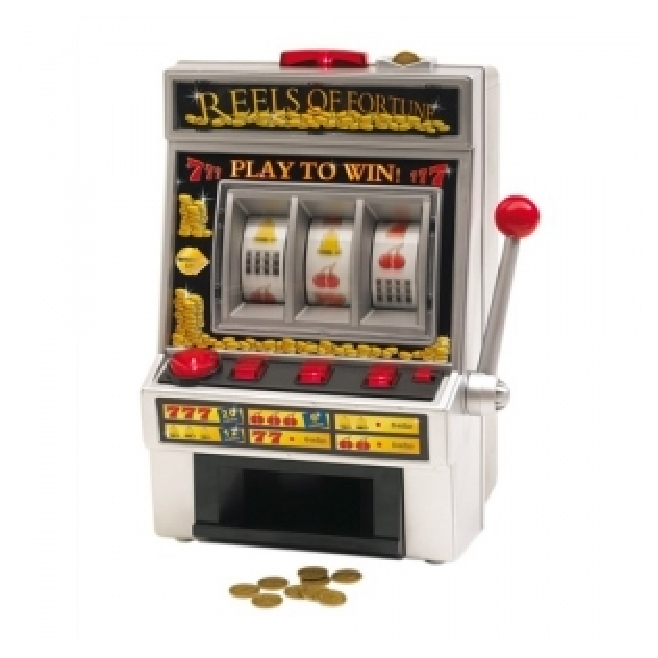
\includegraphics[width=8.0cm]{bandit.eps}
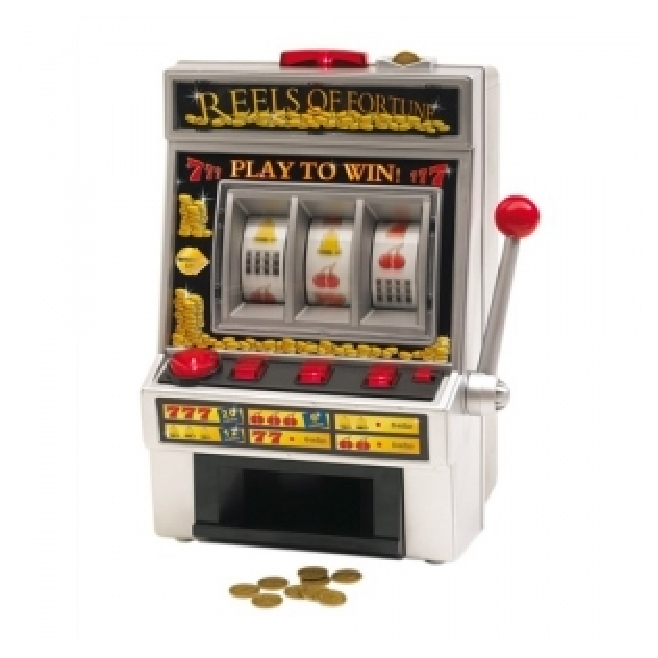
\includegraphics[width=8.0cm]{bandit.eps}
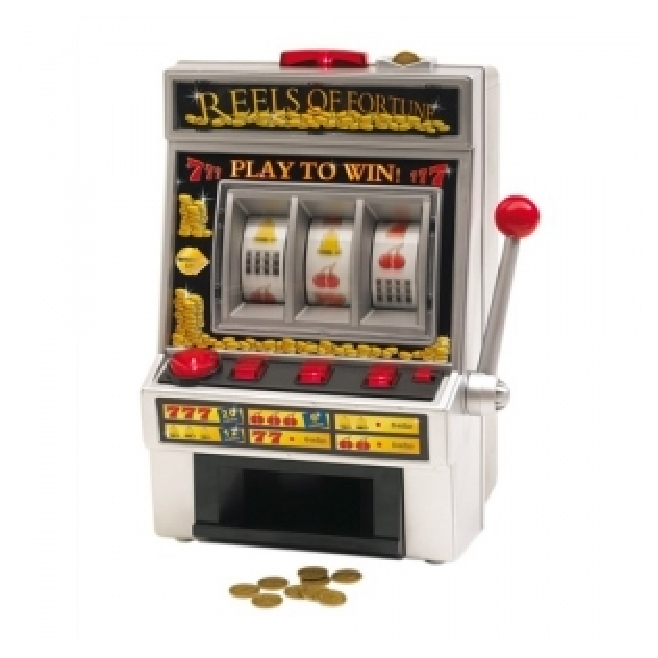
\includegraphics[width=8.0cm]{bandit.eps}


\begin{center}
$K$ one-armed bandit slot machines. 
\end{center}

$\blue \bullet$ At each new timestep the player :

- pulls an arm $i_t$ according to his strategy, which can depend on past observation and be randomized

- observes the reward $r_{i_t}(t)$ of the chosen arm $i_t$ 

$\blue \bullet$ {\bf Stochastic Setting}: rewards are given by stationnary unknown probability distributions $r_i$

$\blue \bullet$ {\bf Adversarial Setting}: an opponent, aware of the player's past decisions and rewards, chooses simultaneously with the player a (possibly randomized)
reward $r_i(t)$ for each arm.

\begin{center}
  What can you do in the adversarial case ?
\end{center}

$\blue \bullet$ impossible to ``maximize'' reward

$\blue \bullet$ You can try to minimize the {\bf external regret}: 
difference at time $T$ between one's gain and
the gain which could have been obtained by allways pulling {\it the same} arm

$$R_T = \max_{i=1\ldots k} \left( \sum_{t=1}^{T} r_i(t) \right) - \sum_{t=1}^T r_{i_t} (t)$$


\begin{center}
  \bf External regret can be minimized (in expectation or with high probability) by the EXP3 Algorithm \cite{auer03}
\end{center}
}
\end{pcolumn}

\vspace{.5cm}
\begin{pcolumn}{0.32}



\pbox{0.9\textwidth}{47cm}{linewidth=2mm,framearc=0.1,linecolor=lightblue,fillstyle=gradient,gradangle=0,gradbegin=white,gradend=white,gradmidpoint=1.0,framesep=1em}{


\vspace{2cm}\begin{center}\pbox{0.8\textwidth}{}{linewidth=2mm,framearc=0.1,linecolor=lightblue,fillstyle=gradient,gradangle=0,gradbegin=white,gradend=whiteblue,gradmidpoint=1.0,framesep=1em}{\begin{center}EXP3 Algorithm\end{center}}\end{center}\vspace{1.25cm}
  {\large
  Parameter : real $\gamma \in ]0;1]$

  Initialization : define the weight $w_i(t)=1$ for $t=1$ and all $i=1,\ldots k$

  For each $t=1,2,\ldots$

  \begin{enumerate}
    \item Set
      $$p_i(t)=(1-\gamma) \frac{w_i(t)}{\sum_{j=1}^k w_j(t)} + \frac{\gamma}{K}$$
      for $i=1,\ldots K$.
    \item Select randomly an arm $i_t$ according the the probabilities $p_1(t), \ldots,p_K(t)$
    \item Observe the reward $r_{i_t}(t)$
    \item Update the weight of $i_t$ by
      $$w_{i_t} (t+1) = w_{i_t} (t) \exp( \frac{\gamma}{K} \frac{ r_{i_t}(t)}{p_{i_t}(t)} )$$
      and set $w_j(t+1)=w_j(t)$ for other arms.
  \end{enumerate}

  \vspace{.3cm}
  
  $\blue \bullet$  
  In order to find good actions EXP3 maintains a balance between 
  
  - { \bf exploration}: weighting actions according to the reward:  $1-\gamma$ term in the probability, and 
  
  - {\bf exploration}: the uniform term $\frac{\gamma}{K}$ ensures that unsufficiently tested actions will be regularly selected.
  

  \vspace{.3cm}
  
  {\bf Theorem} [Auer {\it et al} \cite{auer03}]
  {\it
    When run with parameter $$\gamma=\min{0.8\sqrt{\frac{\ln K}{T K},\frac{1}{K}}}$$
    the expected regret
satisfies 
$$\frac{R_T}{T} \leq 2.7 \sqrt{ \frac{K \ln K}{T} }$$
}

}

}

\end{pcolumn}

\begin{pcolumn}{0.32}
\pbox{0.9\textwidth}{21cm}{linewidth=2mm,framearc=0.1,linecolor=lightblue,fillstyle=gradient,gradangle=0,gradbegin=white,gradend=white,gradmidpoint=1.0,framesep=1em}{

\vspace{2cm}\begin{center}\pbox{0.8\textwidth}{}{linewidth=2mm,framearc=0.1,linecolor=lightblue,fillstyle=gradient,gradangle=0,gradbegin=white,gradend=whiteblue,gradmidpoint=1.0,framesep=1em}{\begin{center}External regret and Zero-Sum Matrix Games\end{center}}\end{center}\vspace{1.25cm}

  $\blue \bullet$ Two players simultaneously choose a column $i$ and a line $j$ of a given matrix $M$ 

  $\blue \bullet$ The line player receives $M_{i,j}$ and the column player receives $-M_{i,j}$.

 
  Exemple : the Rock-Paper-Scissors game

  \[
  \left(
  \begin{array}{c|ccc}
    & \mbox{Rock} & \mbox{Cissors} & \mbox{Paper} \\
    \mbox{Rock} & 0 & +1 & -1 \\
    \mbox{Cissors} & -1 & 0 & +1 \\
    \mbox{Paper} & +1 & 0 & -1 \\
  \end{array} \right)
\]





\begin{center}
 \bf 
If both players repeatedly play,  
selecting their strategies 

with an algorithm minimizing external regret, 

then the empirical frequencies

of play converge to optimal strategies (``Nash Equilibrium'').
\end{center}



}  
\end{pcolumn}

\vspace{.5cm}

\begin{pcolumn}{0.32}
  \pbox{0.9\textwidth}{32cm}{linewidth=2mm,framearc=0.1,linecolor=lightblue,fillstyle=gradient,gradangle=0,gradbegin=white,gradend=white,gradmidpoint=1.0,framesep=1em}{

  \vspace{2cm}\begin{center}\pbox{0.8\textwidth}{}{linewidth=2mm,framearc=0.1,linecolor=lightblue,fillstyle=gradient,gradangle=0,gradbegin=white,gradend=whiteblue,gradmidpoint=1.0,framesep=1em}{\begin{center}Monte-Carlo Tree Search Algorithms\end{center}}\end{center}\vspace{1.25cm}

    $\blue \bullet$ MCTS Algorithms are efficient algorithms designed for tree-searching with huge inputs. 

    $\blue \bullet$ They have been used to design computer players in games with full observation, e.g. Go 

    $\blue \bullet$ Mogo was the first algorithm to win against professional Go players
 
    \begin{center}

      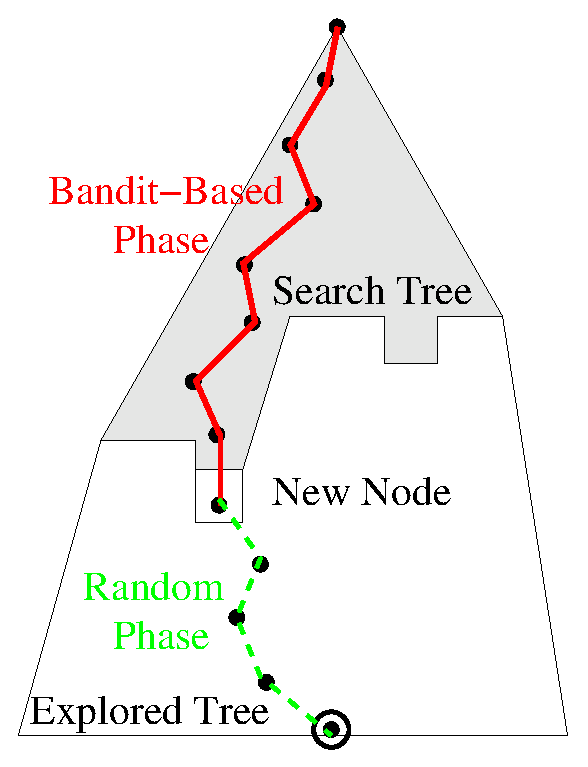
\includegraphics[width=12cm]{mcts.eps}
    \end{center}


       $\blue \bullet$ As in the multi-armed bandit problem we must balance {\it exploitation} and {\it exploration}

       $\blue \bullet$ classical implementations \cite{kocsis06} use the UCB bandit algorithm \cite{lai1985}, designed for the stochastic setting.
    }
  \end{pcolumn}

\vspace{.5cm}

\begin{pcolumn}{0.32}
  \pbox{0.9\textwidth}{29cm}{linewidth=2mm,framearc=0.1,linecolor=lightblue,fillstyle=gradient,gradangle=0,gradbegin=white,gradend=white,gradmidpoint=1.0,framesep=1em}{

  \vspace{2cm}\begin{center}\pbox{0.8\textwidth}{}{linewidth=2mm,framearc=0.1,linecolor=lightblue,fillstyle=gradient,gradangle=0,gradbegin=white,gradend=whiteblue,gradmidpoint=1.0,framesep=1em}{\begin{center}Multiple Tree Monte-Carlo Tree Search \end{center}}\end{center}\vspace{1.25cm}

We propose an adaptation of MCTS algorithms, using EXP3, for partially observable games (e.g. card games) 

    
\includegraphics[width=25cm]{double.eps}

Each player runs a separate MCTS algorithm and sees other players' moves via observations sent by the referee

$\blue \bullet$ in a Player Node ``P'', the player chooses his next action with the EXP3 algorithm

$\blue \bullet$ in an Observation Node ``O'' the player waits for the referee to send an observation


{\bf Properties}: consistant, efficient, online

{\bf Main advantage}: the tree is only partially explored, as opposed to \cite{zink08}
    
}
  \end{pcolumn}


\vspace{.5cm}

\begin{pcolumn}{0.32}
  \pbox{0.9\textwidth}{40cm}{linewidth=2mm,framearc=0.1,linecolor=lightblue,fillstyle=gradient,gradangle=0,gradbegin=white,gradend=white,gradmidpoint=1.0,framesep=1em}{
  

  \vspace{2cm}\begin{center}\pbox{0.8\textwidth}{}{linewidth=2mm,framearc=0.1,linecolor=lightblue,fillstyle=gradient,gradangle=0,gradbegin=white,gradend=whiteblue,gradmidpoint=1.0,framesep=1em}{\begin{center}Application to the game of Phantom Tic-Tac-Toe\end{center}}\end{center}\vspace{1.25cm}

    $\blue \bullet$ Played like standard Tic-Tac-Toe but one does not see where the opponent plays.
    
    $\blue \bullet$ In case of an illegal move the player must play somewhere else

    \begin{center}
      
    
\includegraphics[width=5cm]{fantome.eps}
    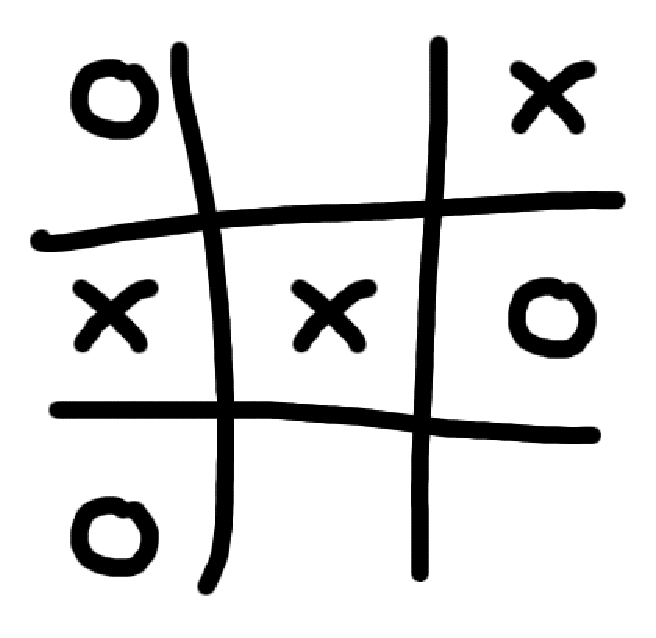
\includegraphics[width=10cm]{tictac.eps}
    
\includegraphics[width=5cm]{fantome.eps}
    \end{center}
    

  Whereas standard Tic-Tac-Toe is a draw, in Phantom Tic-Tac-Toe the first player can force 85 \% of victories with only 4\% of losses.



    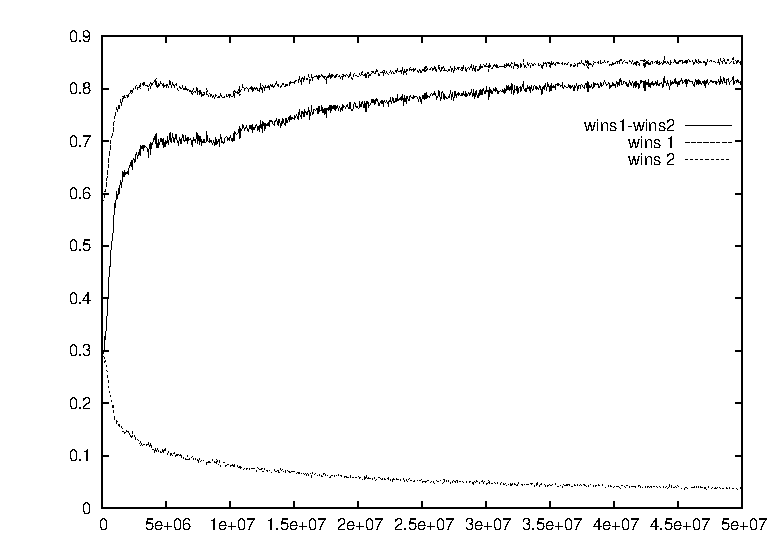
\includegraphics[width=25cm]{1vs2e.eps}
    \begin{center}
      simulations
    \end{center}
    }
  \end{pcolumn}

  
\vspace{.5cm}

\begin{pcolumn}{0.32}
  \pbox{0.9\textwidth}{20cm}{linewidth=2mm,framearc=0.1,linecolor=lightblue,fillstyle=gradient,gradangle=0,gradbegin=white,gradend=white,gradmidpoint=1.0,framesep=1em}{
 
   \vspace{2cm}\begin{center}\pbox{0.8\textwidth}{}{linewidth=2mm,framearc=0.1,linecolor=lightblue,fillstyle=gradient,gradangle=0,gradbegin=white,gradend=whiteblue,gradmidpoint=1.0,framesep=1em}{\begin{center}A Phantom Tic-Tac-Toe personal Olympiad\end{center}}\end{center}\vspace{1.25cm}

Opponents are :

$\blue \bullet$ MMCTS 500K, 5M and 50M, mixed strategies obtained by our algorithm after 500K, 5M or 50M iterations  

$\blue \bullet$ Belief Sampler, who plays standard tic-tac-toe perfectly and randomizes his moves according to optimal strategies
compatible with observations (standard approach for P.O. games, see e.g \cite{cazenave06})

$\blue \bullet$ Random Player, a dummy uniform random player.
\scalebox{.85}{
 \begin{tabular}{|c||c|c|c||c|c|}
   \hline
   P1 \tb \ P2 \ &   MMCTS 500K  &   MMCTS 5M  &   MMCTS 50M  &  Random   &  B.Sampler   \\
   \hline
   \hline
   M.500K                        & $65 \%$ \tb \ $ 25 \%$ & $51 \%$ \tb \ $ 37 \%$ & $44 \%$ \tb \ $ 47 \%$ & $67 \%$ \tb \ $ 22 \%$ & $40 \%$ \tb \ $ 43 \%$\\
   \hline
   M. 5M                          & $88 \%$ \tb \ $ 06 \%$ & $82 \%$ \tb \ $ 10 \%$ & $78 \%$ \tb \ $ 17 \%$ & $88 \%$ \tb \ $ 05 \%$ & $78 \%$ \tb \ $ 10 \%$\\
   \hline
   M. 50M                         & $93 \%$ \tb \ $ 02 \%$ & $89 \%$ \tb \ $ 03 \%$ & $85 \%$ \tb \ $ 04 \%$ & $93 \%$ \tb \ $ 02 \%$ & $82 \%$ \tb \ $ 03 \%$\\
   \hline
   \hline
   Random                            & $55 \%$ \tb \ $ 33 \%$ & $48 \%$ \tb \ $ 39 \%$&$41 \%$ \tb \ $ 47 \%$ & $59 \%$ \tb \ $ 28 \%$ & $30 \%$ \tb \ $ 53 \%$\\
   \hline
   B.Sampler                    & $77 \%$ \tb \ $ 14 \%$ & $73 \%$ \tb \ $ 18 \%$ & $68 \%$ \tb \ $ 22 \%$ & $79 \%$ \tb \ $ 12 \%$ & $56 \%$ \tb \ $ 28 \%$ \\
   \hline
 \end{tabular} 
 }
 %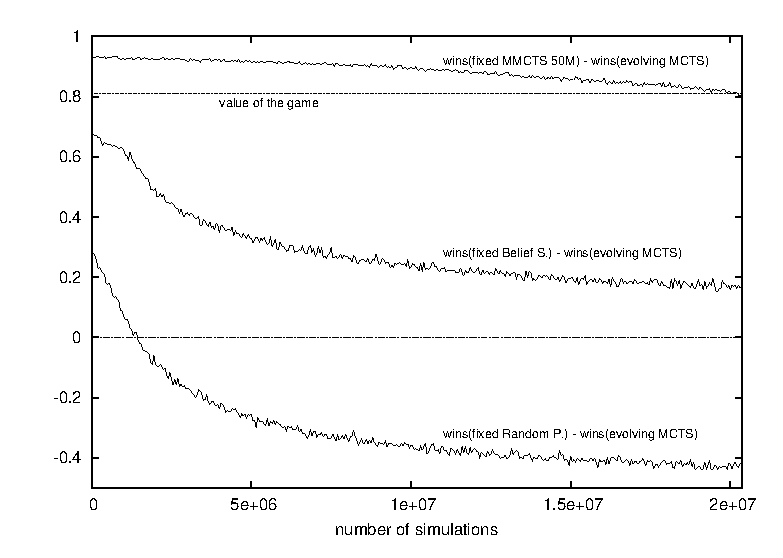
\includegraphics[width=25cm]{nashitude1.eps}
 }
  \end{pcolumn}

\vspace{.5cm}

  \begin{pcolumn}{0.32}
  \pbox{0.9\textwidth}{20cm}{linewidth=2mm,framearc=0.1,linecolor=lightblue,fillstyle=gradient,gradangle=0,gradbegin=white,gradend=white,gradmidpoint=1.0,framesep=1em}{
 
%%% References
    \bibliographystyle{alpha}
    \bibliography{/home/david/Dropbox/biblio/biblio.bib}


  }
\end{pcolumn}


\end{multicols}
%\end{center}

\end{poster}

\end{document}

